\documentclass[a4paper,12pt]{article}
\usepackage[utf8]{inputenc}
\usepackage[russian]{babel}
\usepackage{amsmath}
\usepackage{graphicx}
\usepackage{geometry}
\usepackage{color}
\usepackage{fancyhdr}
\usepackage{titlesec}
\usepackage{setspace}

\geometry{top=2cm,bottom=2cm,left=2cm,right=2cm}

% Настройка заголовков
\titleformat{\section}{\large\bfseries\color{blue}}{}{0em}{}[\titlerule]
\titleformat{\subsection}{\bfseries\color{blue}}{}{0em}{}

% Настройка шапки и подвала
\pagestyle{fancy}
\fancyhf{}
\fancyhead[L]{Классификация распределения с помощью случайных графов}
\fancyhead[R]{\thepage}
\fancyfoot[C]{\textit{Соколовский С.П., Григоренко М.Д.}}

% Настройка интервала между строками
\onehalfspacing

\title{\textbf{Классификация распределения с помощью случайных графов}} 
\author{Соколовский С.П., Григоренко М.Д.}
\date{Дата: \today}

\begin{document}

\maketitle

\section{Предисловие}
Договоримся об обозначениях: \begin{itemize}
    \item $n$ --- размер вектора реализаций случайной величины
    \item $k$, $d$ --- параметры построения KNN и дистанционного графов соответственно
    \item $\theta, v$ --- параметры распределений
    \item $T^{KNN}$, $T^{dist}$ --- характеристики случайных графов
\end{itemize}

\section{Часть I. Исследование свойств характеристики}
\subsubsection*{Используемые инструменты Соколовского С.П.}
Весь код в ветке \texttt{Crazy-Explorer31/first\_part}, в директории \texttt{src/}:
\begin{itemize}
    \item \texttt{graphs.py} --- реализации KNN и дистанционного графов (у каждого есть метод для построения и отрисовки)
    \item \texttt{characteristics.py} --- функции для получения характеристик графов, построенных при данных параметрах (распределений, построения графов...). Самый важный --- \textttt{get\_average\_characteristics}, возвращающий средние характеристики графов, построенных при переданных параметрах
    \item \texttt{visualisations.py} --- функции для удобной построения графиков
    \item \texttt{metrics.py} --- функции, приближенно считающие ошибку I рода и мощность для данного $\mathcal{A}$. Считается по методу Монте-Карло, используя переданное в функцию множество точек (число компонент, хром число), принадлежащих какому-то распределению.
\end{itemize}

\subsubsection*{Используемые инструменты Григоренко М.Д.}
Весь код в ветке \texttt{maxGrigorenko/first\_part}, в директории \texttt{src/}:
\begin{itemize}
    \item \texttt{graph\_common\_functions.py} --- реализации KNN и дистанционного графов (у каждого есть метод для построения из значений случайной величины, а также методы вычисления характеристик)
    \item \texttt{distribution\_functions.py} --- функции для генерации выборки и вычисления матожидания характеристики методом Монте-Карло.
\end{itemize}


\subsection{Шаг 1. Фиксируем $n$. Исследуем взаимосвязь между $\theta, v$ и $T^{KNN}$, $T^{dist}$}
\subsubsection*{Результаты Соколовского С.П.}
В файле \texttt{experiments\_first\_part\_1.ipynb} происходит следующее:
\begin{itemize}
    \item Для каждой тройки (распределение, тип графа, характеристика) перебираются параметры трех перечисленных объектов, после чего вычисляются характеристики полученных графов.
    \item Для каждой тройки строится диаграмма рассеивания, в которой по горизонтальной оси --- параметр распределения, а по вертикальной --- характеристика графа
\end{itemize}
Из графиков заметно, что лишь с дистанционным графом хочется продолжать работать
\subsubsection*{Результаты Григоренко М.Д.}
В файле \texttt{experiments\_first\_part\_1.ipynb} происходит следующее:
\begin{itemize}
    \item Реализованы функции \texttt{plot\_sigma} и \texttt{plot\_beta}, перебирающие значения соответствующих параметров распределений и выводящих график зависимости характеристики графов (knn и dist) от перебираемого параметра
    \item При фиксированном размере выборки проведены эксперименты с различными параметрами $d$ и $k$.
\end{itemize}
В результате всех экпериментов delta графа knn была константной, то есть
эта характеристика никак не связана с параметрами распределений. А вот доминирующее число дистанционного графа в среднем увеличивалось при увеличении параметра sigma. На двух графиках ниже показана зависимость среднего числа характеристик в завимости от параметров распределений: \newline
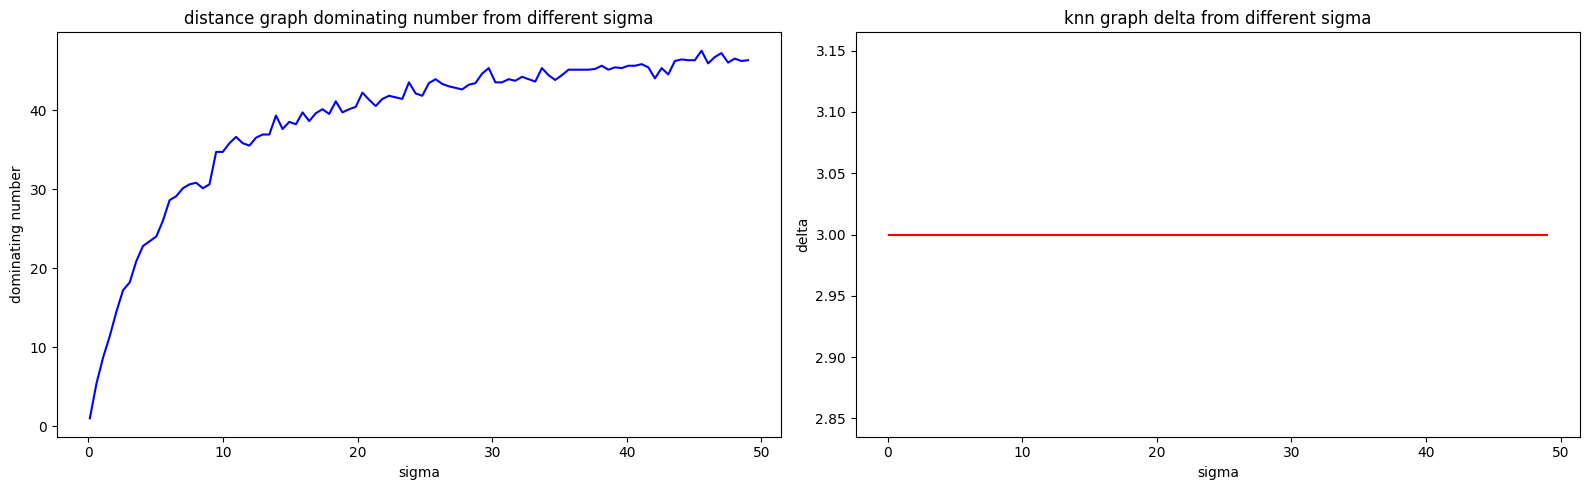
\includegraphics[width=\textwidth]{images/sigma_plot.png} \newline
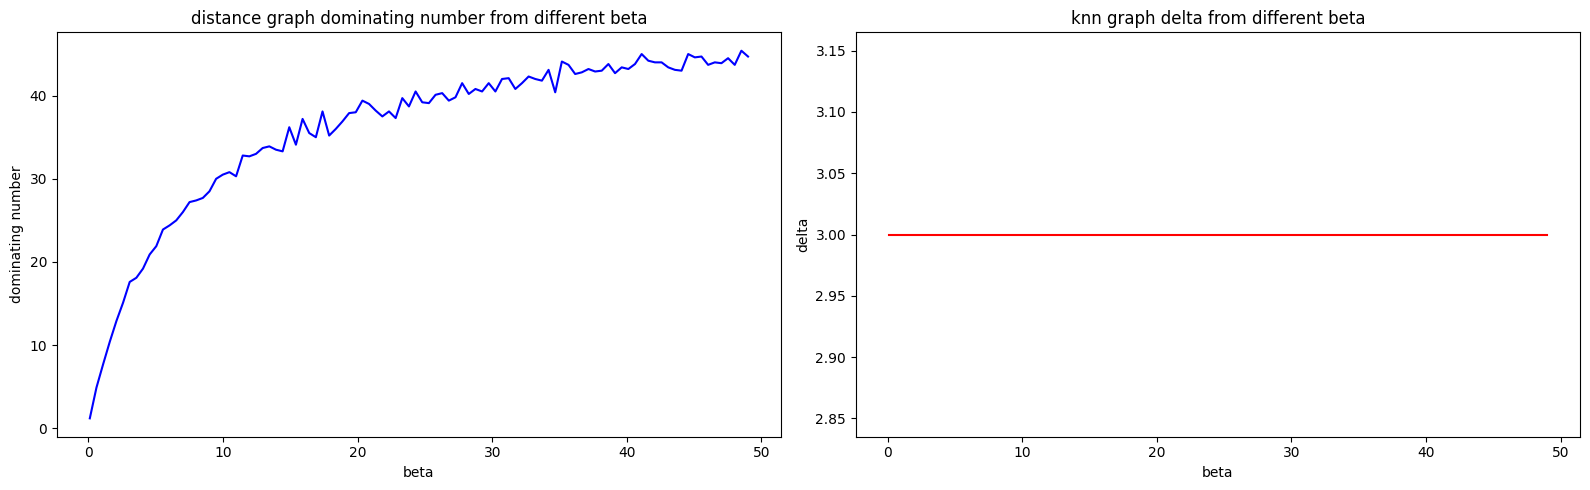
\includegraphics[width=\textwidth]{images/beta_plot.png} \newline

\subsection{Шаг 2. Фиксируем $\theta, v$. Исследуем взаимосвязь между $n$, $k$, $d$ и $T^{KNN}$, $T^{dist}$}
\subsubsection*{Результаты Соколовского С.П.}
В файле \texttt{experiments\_first\_part\_2.ipynb}, аналогично первому шагу, генерятся много налюдений для всех комбинаций распределений, типов графов, их характеристик. Далее на диаграммах рассеивания по оси Ox откладываются параметры построения графов, по Oy --- их характеристики, и ещё цветом отражена, при каком $n$ было получено наюлюдение. Выводы аналогичные первому эксперименту
\subsubsection*{Результаты Григоренко М.Д.}
В файле \texttt{experiments\_first\_part\_2.ipynb} зафиксированы параметры распределений и отрисованы графики зависимости характеристик графов от размера выборки. delta графа knn оказалась неинформативной характеристикой. А вот доминирующее число дистанционного графа немного по-разному меняется при изменении размера выборки, в особенности, если в качестве параметра дистанционного графа установить значение $d >= 3$, то характеристика графа из нормального распределения становится почти всегда равной 1, а вот при распределении Лапласа немного больше. Снизу график зависимости среднего числа доминирования от размера выборки при $d = 3.5$: \newline
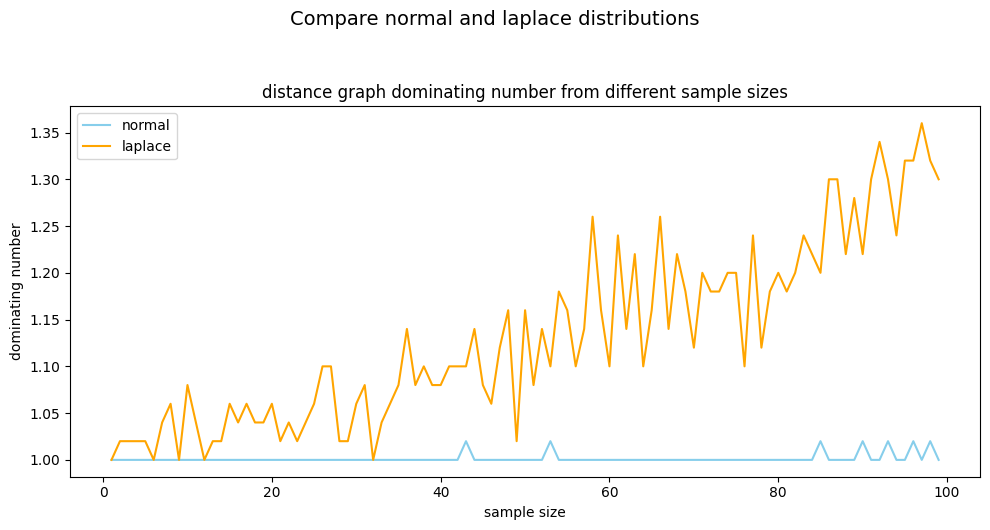
\includegraphics[width=\textwidth]{images/dominating_number_plot.png}

\subsection{Шаг 3. Фиксируем $\theta, v$. Строим $\mathcal{A}$ для переданного $n$}
\subsubsection*{Результаты Соколовского С.П.}
Файл \texttt{experiments\_first\_part\_3.ipynb} поделен на два раздела. В первом фиксируются все параметры и строится $\mathcal{A}$. Во втором рассуждения, изложенные в первом разделе обобщаются, и приведена реализация класса, строящая $\mathcal{A}$ по переданному в конструктор $n$ \\
Используется следующий алгоритм построения $\mathcal{A}$:
\begin{itemize}
    \item[1.] Строятся точки с координатами (число компонент, хроматическое число) по генерирующимся векторам случайных величин
    \item[2.] За изначальное $\mathcal{A}$ берется множество всех сгенерированных точек, полученных по первому распределению (Exp).
    \item[3.] Далее пытаемся удалить точку из $\mathcal{A}$ так, чтобы ошибка I рода не превысила 0.05, а мощность была максимальной (ошибка I рода и мощность считаются на основе точек, сгенерированных в начале). Для этого перебираем все варианты и выбираем наилучший
    \item[4.] Пытаемся так удалить что-то из $\mathcal{A}$ много раз
    \item[5.] В итоге получаем искомое $\mathcal{A}$
\end{itemize}
\subsubsection*{Результаты Григоренко М.Д.}
В файле \texttt{experiments\_first\_part\_3.ipynb} реализован алгоритм конструирования множества $\mathcal{A}$, которое должно удовлетворять двум условиям:

\begin{itemize}
\item[1.] Контроль ошибки первого рода: вероятность ошибочно отвергнуть нулевую гипотезу $H_0$ (данные имеют нормальное распределение) при её справедливости не превышает $\alpha = 0.05$.

\item[2.] Максимизация мощности: вероятность корректно отвергнуть $H_0$ в пользу альтернативы $H_1$ (например, распределение Лапласа) должна быть максимальной.
\end{itemize}

Множество $\mathcal{A}$ конструируется итеративно следующим образом:
На каждом шаге генерируется большое число выборок (number\_of\_experiments) из нормального распределения. Для каждой выборки вычисляется характеристика графа. Если значение характеристики не принадлежит текущему множеству $\mathcal{A}$, оно считается "ошибочным" (ложным отклонением $H_0$). Ошибка первого рода оценивается как доля таких "ошибочных" случаев:
Пока ошибка $\text{err} > \alpha$, в $\mathcal{A}$ добавляется наиболее частое значение характеристики из "ошибочных" результатов (мода). Это снижает долю ошибок за счёт включения типичных для $H_0$ значений.
Процесс останавливается, когда $\text{err} \leq \alpha$, либо когда "ошибочные" значения исчерпаны.

\section{Часть II. Несколько характеристик проверки гипотезы}
\subsection{Шаг 1. Исследуем важность характиристик}
\subsubsection*{Результаты Соколовского С.П.}
TODO

\subsubsection*{Результаты Григоренко М.Д.}
В файле \texttt{experiments\_second\_part.ipynb} написан класс \texttt{DistribituionClassifier}, принимающий на вход параметр $n$ - размер выборки и модель классификации, которую предстоит обучить. Для выявление признаков по данной выборке строится 4 дистанционных графа с различным параметром $d$, для каждого графа считаеются следующие характеристики:
\begin{itemize}
    \item[1.] Минимальная степень вершины
    \item[2.] Средняя степень вершины
    \item[3.] Максимальная степень вершины
    \item[4.] Число доминирования
    \item[5.] Кликовое число
\end{itemize}
TODO

\subsection{Шаг 2. Метрики качества для разных выборок}
\subsubsection*{Результаты Соколовского С.П.}
TODO

\subsubsection*{Результаты Григоренко М.Д.}
TODO

\subsection{Шаг 3. Выводы о вероятности ошибки первого рода и мощности подхода}
\subsubsection*{Результаты Соколовского С.П.}
TODO

\subsubsection*{Результаты Григоренко М.Д.}
TODO


\end{document}